Ionic conductors are a unique class of solid-state materials which contain mobile ions, that are not spatially confined to particular lattice sites, but act as mobile ions that move across the lattices, conducting both masses and charges through the systems. Determining the ionic conductivities plays an important role in understanding the physical properties, and helps in the design of functional materials, including, for instances, (a) the search for fast ion conductors for safe and compact solid-state electrolytes,\cite{bachman2016inorganic} (b) enhancing the hydrogen storage capabilities in the solid-state hydrogen storage materials,\cite{berube2007size} (c) the stabilities of mixed halide perovskite photovoltaic materials against photo-induced phase segregations,\cite{hu2022valence} (d) ionic contribution to the Seebeck coefficients in  ionic thermoelectrics,\cite{song2022ionic} and (e) the formation and stabilities of oxygen vacancies, which dictate the ferroelectric properties of perovskites.\cite{yang2013strain}

\begin{figure}[htb]
    \centering
    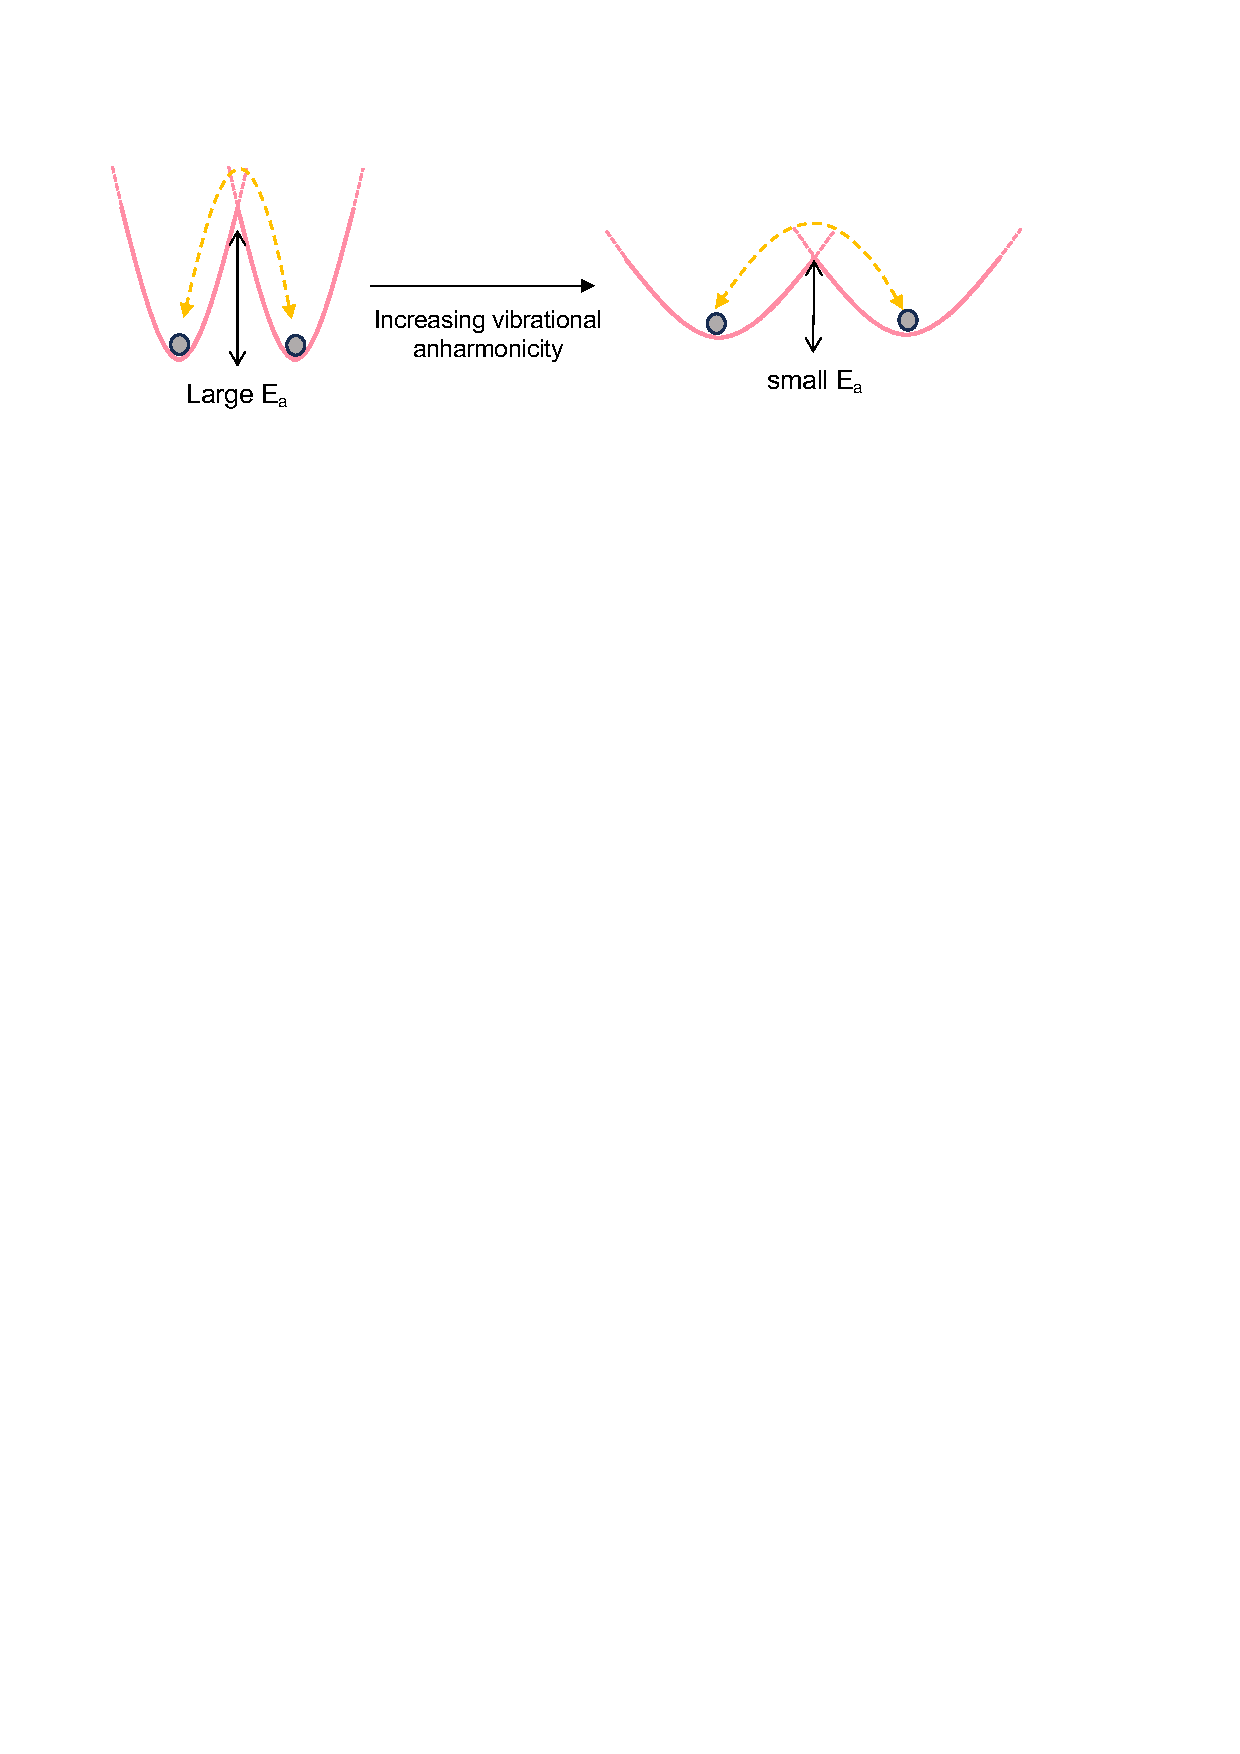
\includegraphics[width=0.7\linewidth]{anharmonic_diffusion.pdf}
    \caption{Schematic illustration of how softening of the lattice, which enhances the vibrational anharmonicity, reduces the activation energy $E_a$ for ion diffusions, leading to an enhancement in the corresponding ion diffusivity.}
    \label{fig:anharmonic_diffusion}
\end{figure}

Fundamentally, ions diffuse through a periodic lattice by hopping between two adjacent local minima on the PES [\cref{fig:anharmonic_diffusion}(left)] that are separated by an energy barrier, which is commonly referred to as the activation energy $E_{a}$. Typically, when the mobile ions diffuse through the lattice, they need to `push' away their surrounding atoms by overcoming the repulsive forces with these surrounding atoms to open up the diffusion pathway, such that $E_{a}$ is strongly correlated with the strengths of these repulsive interactions. If one assumes the host lattice is frozen, then the thermal energy is primarily contributing for the mobile ions to overcome the activation energy in achieving the hopping between two adjacent local minima, such that the temperature-dependent ion diffusivity  $D(T)$ can be determined  by the Arrhenius relationship:
\begin{equation}
    \label{eq:arrhenius_eq}
    D(T)=D_0\exp\left(-\frac{E_a}{k_B T}\right).
\end{equation}
However, in reality, the diffusion of the mobile ions are strongly coupled with the vibration of the host lattice to achieve fast ion conduction, in which many different material-specific mechanisms behind such coupling have been proposed.\cite{jun2024diffusion} More specifically, with respect to the above discussions on the anharmonic lattice vibrations, it is commonly understood that anharmonicity flattens the PES, thus reducing the $E_{a}$ to promote fast ion conduction in solids [\cref{fig:anharmonic_diffusion}(right)]. 

Practically, the ion conductivity ($\sigma$) is often the measured experimental quantity that characterises the performance of ionic conductors, which relates to the ion diffusivity via the Einstein relationship $\sigma=nq^2D/k_B T$, in which $n$ is the concentration of the charge carriers and $q$ is the associated charge. From here, it is not difficult to appreciate that, being able to determine the ion diffusivity $D$ will be the key in applying computational methodologies to supplement experimental results in understanding the mechanisms behind fast ion conduction in solids. Computationally, $D(T)$ can be computed from MD simulations at a constant temperature $T$ via the mean-squared-displacements (MSD) of ions over the simulation time:
\begin{equation}
    \label{eq:ion_MSD}
    D(T)=\lim_{t\to \infty}\frac{1}{6Nt}\sum_{i=1}^{N}\left\langle \left\vert \bm{R}_i(t)-\bm{R}_i(0) \right\vert^2\right\rangle.
\end{equation}
In addition, MD simulations are capable of providing a rich set of structural information which is particularly useful for identifying the most likely ionic conduction pathway in materials. This information can be further utilised to conduct further theoretical modelling, for example, with the Nudged Elastic Band (NEB) method, to map out the detailed PES along the ion diffusion pathway,\cite{he2017origin} from which not only the corresponding $E_a$ can be determined, but also obtain more detailed atomistic insights on the atomic interactions that lead to a high/low $E_a$ along a particular ion conduction pathway. Further supplementing MD simulations with harmonic phonon calculations could help identify vibrational modes that couple strongly with the conduction of mobile ions, of which anharmonic vibrations may play a significant role in contributing towards the fast ion conduction in the system.
